\section{Métricas de validación}
% TODO Corrección [2]: Añadir párrafo introductorio resaltando el marco integrado: segmentación (F1, mAP@50, mAP@50-95) + tracking (HOTA, AssA, IDF1, MOTA, MT%, IDSW, Frag) como contribución metodológica.
% TODO Corrección [14]: Esta sección se moverá / referenciará dentro del nuevo Capítulo 4 (Validación) tras reestructuración.
Para determinar el rendimiento de un modelo es necesario obtener métricas de validación específicas para cada tarea. En el caso de la segmentación de instancias, las métricas más utilizadas son el \textit{mean average precision} (mAP) y el \textit{F1 score}. En este trabajo se priorizó la optimización de la métrica mAP@50-95, que corresponde al promedio de la precisión media calculada en umbrales de IoU desde 0.50 hasta 0.95, en pasos de 0.05.

 En la tarea de seguimiento existen varias métricas bien establecidas en la literatura. Las más tradicionales son MOTA y MOTP, pero en los últimos años han surgido métricas (p. ej. HOTA, AssA, IDF1) que descomponen el rendimiento en detección y asociación, por lo que resultan más informativas para problemas donde la conservación de identidad y la continuidad del seguimiento son prioritarias ---como en este trabajo.

 En consecuencia, aunque en la literatura se reporta con frecuencia MOTA, en este trabajo se priorizan métricas que directamente miden la calidad de la asociación (AssA / IDF1) y la continuidad de tracks (MT / MT\%), y se utiliza HOTA (y sus subcomponentes) para obtener una visión balanceada entre detección y asociación. MOTA se calcula y se muestra por completitud pero no es la métrica de decisión principal, porque puede enmascarar mejoras en la asociación cuando el detector cambia el balance FP/FN.
% TODO Corrección [11]: Matizar este párrafo: reconocer valor de MOTA para medir calidad global de asociaciones y justificar uso complementario en lugar de restarle importancia.

\subsection{Matriz de confusión}
La matriz de confusión ---también conocida como matriz de errores o matriz de coincidencias--- es una representación tabular que muestra, de forma simultánea, los aciertos y errores de un clasificador. Cada fila corresponde a la clase real de los ejemplos y cada columna a la clase predicha, lo que permite evaluar de un vistazo la capacidad del modelo para distinguir entre \textbf{verdaderos positivos}, \textbf{falsos positivos}, \textbf{falsos negativos} y \textbf{verdaderos negativos}.

\begin{table}[htbp]
\centering
\small
\caption[Matriz de confusión]{Matriz de confusión. \cite{TableOfConfusion-Wikipedia}}
\label{tab:confusion_matrix}
\begin{tabular}{|c|c|c|}
\hline
\begin{tabular}[c]{@{}c@{}}Población total\\ (P + N)\end{tabular} &
  Predicho positivo &
  Predicho negativo \\ \hline
\begin{tabular}[c]{@{}c@{}}Real positivo\\ (P)\end{tabular} &
  \begin{tabular}[c]{@{}c@{}}Verdadero positivo\\ (VP o TP)\\ \footnotesize{\textit{Acierto o hit.}}\end{tabular} &
  \begin{tabular}[c]{@{}c@{}}Falso negativo\\ (FN)\\  \footnotesize{\textit{Fallo o miss}}\\  \footnotesize{\textit{(subestimación).}}\end{tabular} \\ \hline
\begin{tabular}[c]{@{}c@{}}Real negativo\\ (N)\end{tabular} &
  \begin{tabular}[c]{@{}c@{}}Falso positivo\\ (FP)\\  \footnotesize{\textit{Falsa alarma}}\\  \footnotesize{\textit{(sobrestimación).}}\end{tabular} &
  \begin{tabular}[c]{@{}c@{}}Verdadero negativo\\ (VN o TP)\\  \footnotesize{\textit{Rechazo correcto.}}\end{tabular} \\ \hline
\end{tabular}
\end{table}

\subsection{Intersección sobre unión (IoU)}
Se define como el area de intersección, dividida por el área de la unión entre la segmentación predicha por el modelo ($S_p$) y la segmentación real o \textit{ground-truth} ($S_{gt}$) (Ec. \ref{eq:intersection_over_union}).

\begin{equation}
  \label{eq:intersection_over_union}
\text{IoU} = \dfrac{\acute{a}rea\left(S_{p} \cap S_{gt}\right)}{\acute{a}rea\left(S_{p} \cup S_{gt}\right)}
\end{equation}

\begin{figure}[htbp]
\begin{center}
    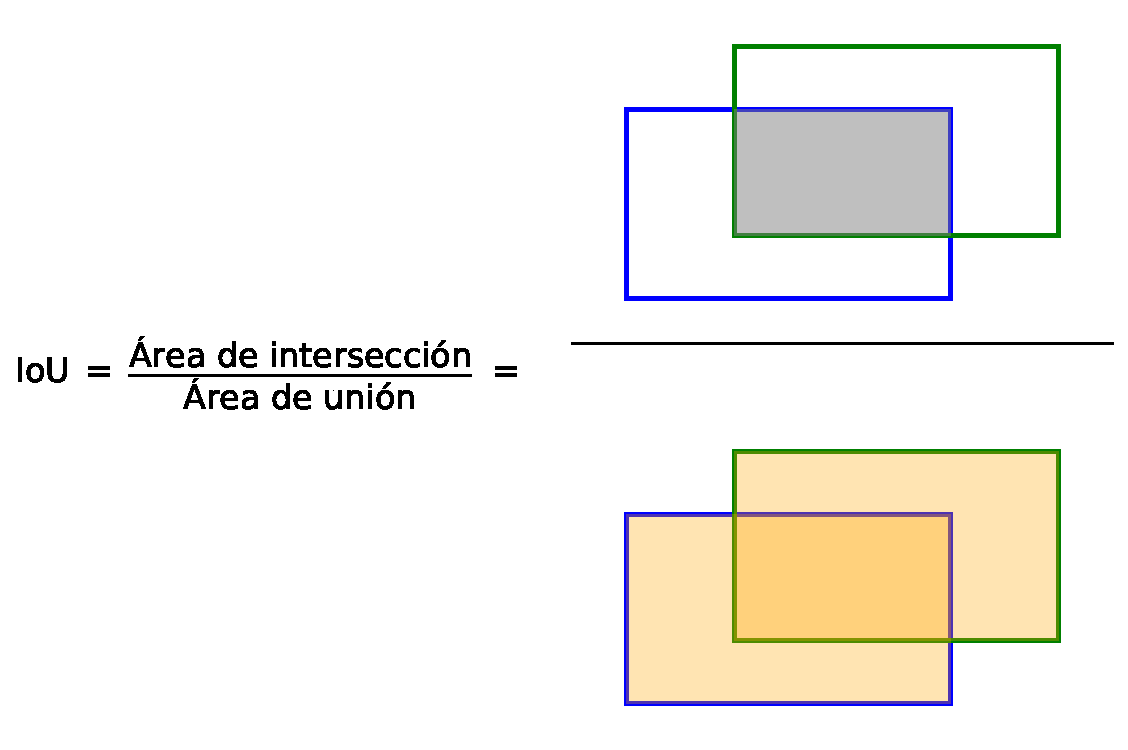
\includegraphics[width=0.6\textwidth]{figures/IoU.pdf}
    \caption[Intersección sobre la unión (IoU)]{Intersección sobre la unión.}
    \label{fig:intersection_over_union}
\end{center}
\end{figure}

El uso de IoU permite clasificar el tipo de predicción realizada. Comúnmente se emplea un umbral del 50\% o 75\% para considerar una predicción como \textbf{verdadero positivo}. A partir de la matriz de confusión obtenida, es posible calcular diversas métricas de rendimiento.

\subsection{Precisión y exhaustividad}
La precisión se define como la proporción de instancias recuperadas que son realmente relevantes, mientras que la exhaustividad (también conocida como sensibilidad o \textit{recall}) corresponde a la fracción de instancias relevantes que han sido correctamente recuperadas. En el contexto del aprendizaje automático, se consideran instancias relevantes aquellas que pertenecen a la clase buscada (\textbf{verdaderos positivos} y \textbf{falsos negativos}), y como instancias recuperadas todas las predicciones realizadas (\textbf{verdaderos positivos} y \textbf{falsos positivos}). Estas relaciones se expresan en las ecuaciones \ref{eq:precision} y \ref{eq:recall}.%, y se ilustran en la figura \ref{fig:presicion_recall}.

\begin{equation}
\text{Precisión} = \dfrac{VP}{VP + FP}
\label{eq:precision}
\end{equation}
\begin{equation}
\text{Recall} = \dfrac{VP}{VP + FN}
\label{eq:recall}
\end{equation}

%\begin{figure}[htbp]
%\begin{center}
%    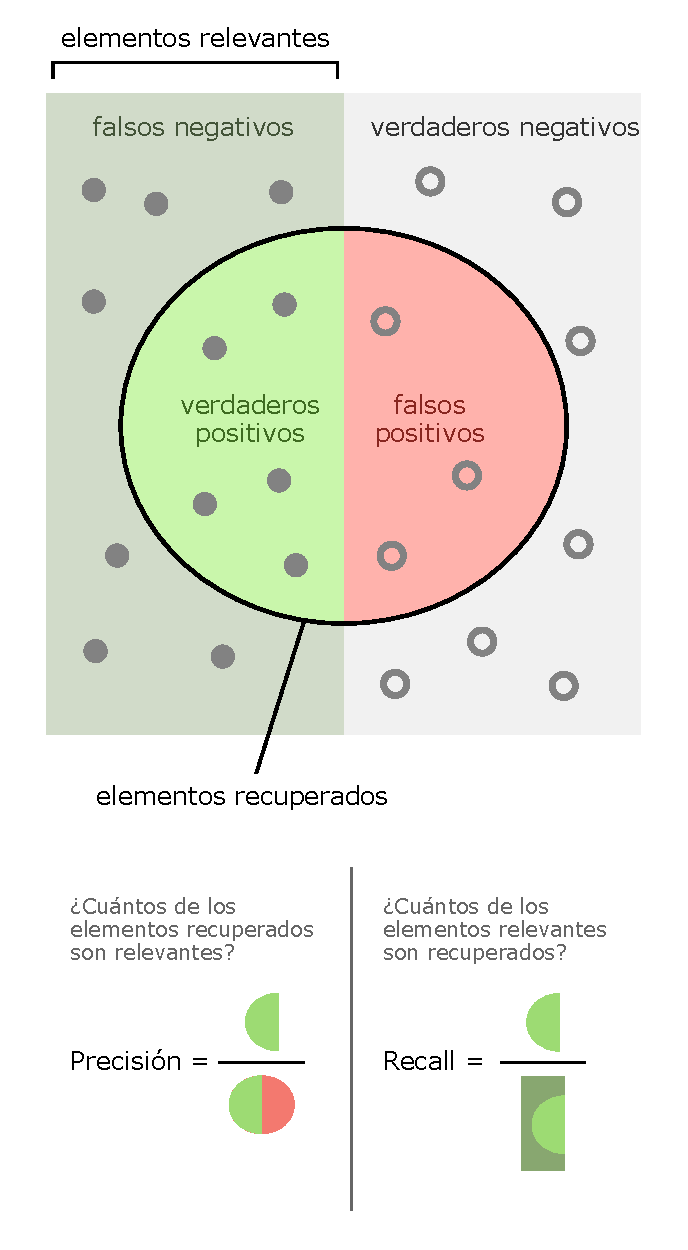
\includegraphics[width=0.55\textwidth]{figures/Precisionrecall_es.pdf}
%    \caption[Presición y exhaustividad]{Presición y exhaustividad (\textit{recall}).}
%    \label{fig:presicion_recall}
%\end{center}
%\end{figure}


\subsection{Puntaje F1}
El puntaje F1 es una métrica que combina la precisión y la exhaustividad en un único valor, proporcionando un equilibrio entre ambas. Se define como la media armónica de la precisión y la exhaustividad, y se calcula mediante la siguiente ecuación (Ec. \ref{eq:f1_score}). El puntaje F1 es especialmente útil en clasificación binaria, donde solo importa distinguir entre una clase y el fondo.

\begin{equation}
\text{F1} = 2 \cdot \dfrac{\text{Precisión} \cdot \text{Recall}}{\text{Precisión} + \text{Recall}}
\label{eq:f1_score}
\end{equation}

\subsection{Mean average precision (mAP)}
La \textit{mean average precision} (mAP) es el promedio de la precisión media de cada clase para una tarea de clasificación y es comúnmente utilizada para evaluar el rendimiento de modelos de detección de objetos y segmentación de instancias, ya que proporciona una medida global del rendimiento del modelo en todas las clases \cite{v7labs-mAP}.

Aunque en esta memoria se trabajó con bases de datos mono-clase, lo que implica que los puntajes mAP y F1 pueden arrojar resultados similares al validar los modelos entrenados, el mAP ofrece una ventaja adicional al considerar la curva precisión-exhaustividad completa a diferentes umbrales. Además Ultralytics no calcula el puntaje F1 y este debe ser obtenido manualmente utilizando los valores de \textit{precision} y \textit{recall} que fueron obtenidos con un umbral IoU fijo del 60\%.

Se calcula mediante la siguiente ecuación (Ec. \ref{eq:map}):

\begin{equation}
\text{mAP} = \dfrac{1}{N} \sum_{i=1}^{N} \text{AP}_i
\label{eq:map}
\end{equation}

donde $N$ es el número de clases y $\text{AP}_i$ es la precisión media de la clase $i$. La precisión media se calcula como el área bajo la curva de precisión-exhaustividad (PR) para cada clase, y se define como el promedio de la precisión en diferentes puntos de \textit{recall}. 

% TODO: Falta agregar fuentes y citas para las métricas de tracking.
% TODO Corrección [13]: Completar referencias formales para IDF1, MOTA/MOTP, MT/PT/ML, IDSW, Frag y AssA (además de HOTA ya citada). Incluir resultados de MOTA en tablas de resultados.
\subsection{HOTA, DetA, AssA y LocA}
HOTA \cite{HOTA} (\textit{Higher Order Tracking Accuracy}) es una métrica de seguimiento que busca equilibrar detección y asociación. HOTA y sus subcomponentes se obtienen emparejando detecciones y \textit{ground-truths} por cuadro (usualmente por IoU) y calculando las razones TP/FP/FN y medidas de asociación por umbral. Es habitual reportar HOTA como AUC (\textit{Area Under the Curve}) sobre distintos umbrales IoU. En la práctica se reporta:
\begin{itemize}
  \item \textbf{DetA (Detection Accuracy)}: métrica de detección (combina TP/FP/FN) en un punto de coincidencia dado.
  \item \textbf{AssA (Association Accuracy)}: mide la calidad con la que el \textit{tracker} conserva identidades a lo largo de los cuadros.
  \item \textbf{LocA (Localization Accuracy)}: refleja la precisión espacial (IoU / distancia) de las correspondencias verdaderas positivas.
\end{itemize}

\subsection{AssA y AssA\_AUC}
AssA (\textit{Association Accuracy}) mide la calidad de la asociación (capacidad de mantener la misma ID a lo largo del tiempo). Se obtiene para cada par detección-GT correctamente emparejado y se evalúa la consistencia de la identidad; se calcula el puntaje de asociación y, para robustez frente a diferentes umbrales de IoU, se reporta el área bajo la curva (AssA\_AUC).  
%Se utiliza porque captura directamente el objetivo esencial de este trabajo —reducir el ``parpadeo'' y conservar identidades de peces que interesa medir.

\subsection{IDF1}
Es el \textit{F1-score} entre las correspondencias de identidad (ID verdadero positivos, ID falsos positivos, ID falsos negativos). Se computan coincidencias de identidad cuadro-a-cuadro y se calcula precisión/\textit{recall} a nivel de ID. Se calcula con la siguiente fórmula (Ec. \ref{eq:idf1}):
\begin{equation}
\text{IDF1} = \frac{2 \cdot \text{IDTP}}{2\cdot\text{IDTP} + \text{IDFP} + \text{IDFN}}
\label{eq:idf1}
\end{equation}

Se utiliza por ser un indicador directo de la calidad global de las IDs, complementario a AssA y fácil de interpretar.

\subsection{MT, PT, ML (Mostly/Partly/Lost tracked) y MT\%}
Por cada GT (\textit{Ground Truth}) se clasifica su seguimiento como:
\begin{itemize}
  \item \textbf{MT:} \textit{mostly tracked} ---el GT fue detectado en la mayor parte de sus \textit{frames} (p. ej. $>80\%$).
  \item \textbf{PT:} \textit{partly tracked} ---detectado en una fracción intermedia.
  \item \textbf{ML:} \textit{mostly lost} ---detectado en muy pocos \textit{frames}.
\end{itemize}

MT\% es la fracción de GTs que son \textit{mostly tracked}. Se obtiene comparando, para cada GT, el número de cuadros donde existe una correspondencia válida con detecciones; se aplica un umbral de fracción (p. ej. 0.8) para clasificar. Se utiliza por ser una medida de continuidad a lo largo de múltiples cuadros.

\subsection{IDSW (ID switches) y Fragmentación (Frag)}
IDSW cuenta cuántas veces un mismo GT cambia de ID asignada por el \textit{tracker} (indicador de pérdida de identidad). Frag cuenta las rupturas de un seguimiento (un GT aparecía, desaparecía y luego reaparecía como nuevo track). Se obtienen a partir del seguimiento cuadro-a-cuadro tras el emparejamiento; cada cambio de ID o separación de continuidas se suma. Se usan por ser medidas directas del ``parpadeo'' y de la calidad práctica del seguimiento.

\subsection{MOTA y MOTP}
MOTA y MOTP son métricas clásicas en seguimiento. MOTA combina errores de falsos negativos, falsos positivos y cambios de identidad (IDSW) en un solo puntaje, reflejando la precisión global del seguimiento (Ec. \ref{eq:mota}). MOTP mide la precisión espacial de las detecciones emparejadas, reflejando qué tan cerca están las predicciones de las posiciones reales. En esencia, MOTA resume la capacidad del sistema para detectar y seguir objetos correctamente, mientras que MOTP evalúa la exactitud de las posiciones predichas.

\begin{equation}
\text{MOTA} = 1 - \dfrac{\text{FN} + \text{FP} + \text{IDSW}}{\text{Total GT detections}}
\label{eq:mota}
\end{equation}

%\textbf{Limitación:} MOTA agrega errores distintos en un solo número; un detector muy conservador (baja FP) puede mejorar MOTA aunque empeore la asociación. Por ello MOTA es útil como resumen pero \emph{no} suficientemente diagnóstica para decidir en problemas donde la continuidad e identidad son críticas.  
%Se reporta MOTA/MOTP por completitud, pero la selección de modelo se basa principalmente en AssA/IDF1/MT\% y HOTA (y en el análisis por componente de HOTA).

%\subsection{Detección: Precisión, Recall y curvas AUC}
%Las métricas clásicas de detección (Precision, Recall, AP/mAP) siguen siendo %relevantes para verificar que no se sacrifica demasiado recall al mejorar %asociación.  
%\begin{itemize}
%  \item \textbf{Precision / Recall:} fórmulas estándar (Ec. \ref{eq:precision}, %\ref{eq:recall} en este documento).
%  \item \textbf{AP / mAP:} área bajo la curva precision–recall; se usa para %comprobar la capacidad detectora en distintos umbrales.
%\end{itemize}
%\textbf{Por qué se mantienen:} si la asociación mejora pero el detector deja de %encontrar consistentemente los peces de interés, el pipeline de masa/volumen se %vería afectado; por eso se usan conjuntamente con las métricas de tracking.

\subsection{Métricas de comparación}
Estas métricas se utilizan para comparar el rendimiento entre diferentes configuraciones de entrenamiento, modelos o bases de datos.

\subsubsection{Diferencia}
Es simplemente la diferencia entre el valor de una métrica obtenida con una configuración específica y el valor de la misma métrica obtenida con una configuración de referencia. Se calcula mediante la siguiente ecuación (Ec. \ref{eq:difference}):

\begin{equation}
  \text{Diferencia} = \text{Métrica 2} - \text{Métrica 1}
  \label{eq:difference}
\end{equation}

\subsubsection{Mejora relativa}
La mejora relativa se define como la razón de la diferencia entre el valor de una métrica obtenida con una configuración específica y el valor de la misma métrica obtenida con una configuración de referencia, dividida por el valor de la métrica de referencia, todo eso multiplicado por 100. Se calcula mediante la siguiente ecuación (Ec. \ref{eq:relative_improvement}):

\begin{equation}
  \text{Mejora relativa} = 100 \cdot \dfrac{\text{Métrica 2} - \text{Métrica 1}}{\text{Métrica 2}}
  \label{eq:relative_improvement}
\end{equation}

\subsubsection{Factor de mejora}
El factor de mejora se define como la relación entre el valor de una métrica obtenida con una configuración específica y el valor de la misma métrica obtenida con una configuración de referencia. Se calcula mediante la siguiente ecuación (Ec. \ref{eq:improvement_factor}):

\begin{equation}
  \text{Factor de mejora} = \dfrac{\text{Métrica 2}}{\text{Métrica 1}}
  \label{eq:improvement_factor}
\end{equation}